\section{Руководство пользователя программного средства}
\label{sec:manual}

В данном разделе приведены основные сведения по работе с программным средством.

При первом открытии приложения перед пользователем отображается экран, состоящий из трёх вкладок: <<Транзакции>>, <<Счета>> и <<Категории>>.
Сразу после запуска активна вкладка <<Транзакции>>, где отображена история транзакций по дням (см. рисунок~\ref{fig:manual:lists}а).
Для перехода между вкладками можно использовать перелистывания влево и вправо, а также нажатиями на заголовки вкладок.
На вкладке <<Счета>> помимо списка счетов снизу отображаются сводные значения по счетам, такие как сумма всех счетов и среднее число денег в день до ближайшего поступления денег (см. рисунок~\ref{fig:manual:lists}б).
Вкладка <<Категории>> имеет переключатель между категориями расходов и доходов (см. рисунок~\ref{fig:manual:lists}в).
Также рядом в каждом элементе списка отображена статистика по данной категории за всё время.

\begin{figure}[H]
    \centering
    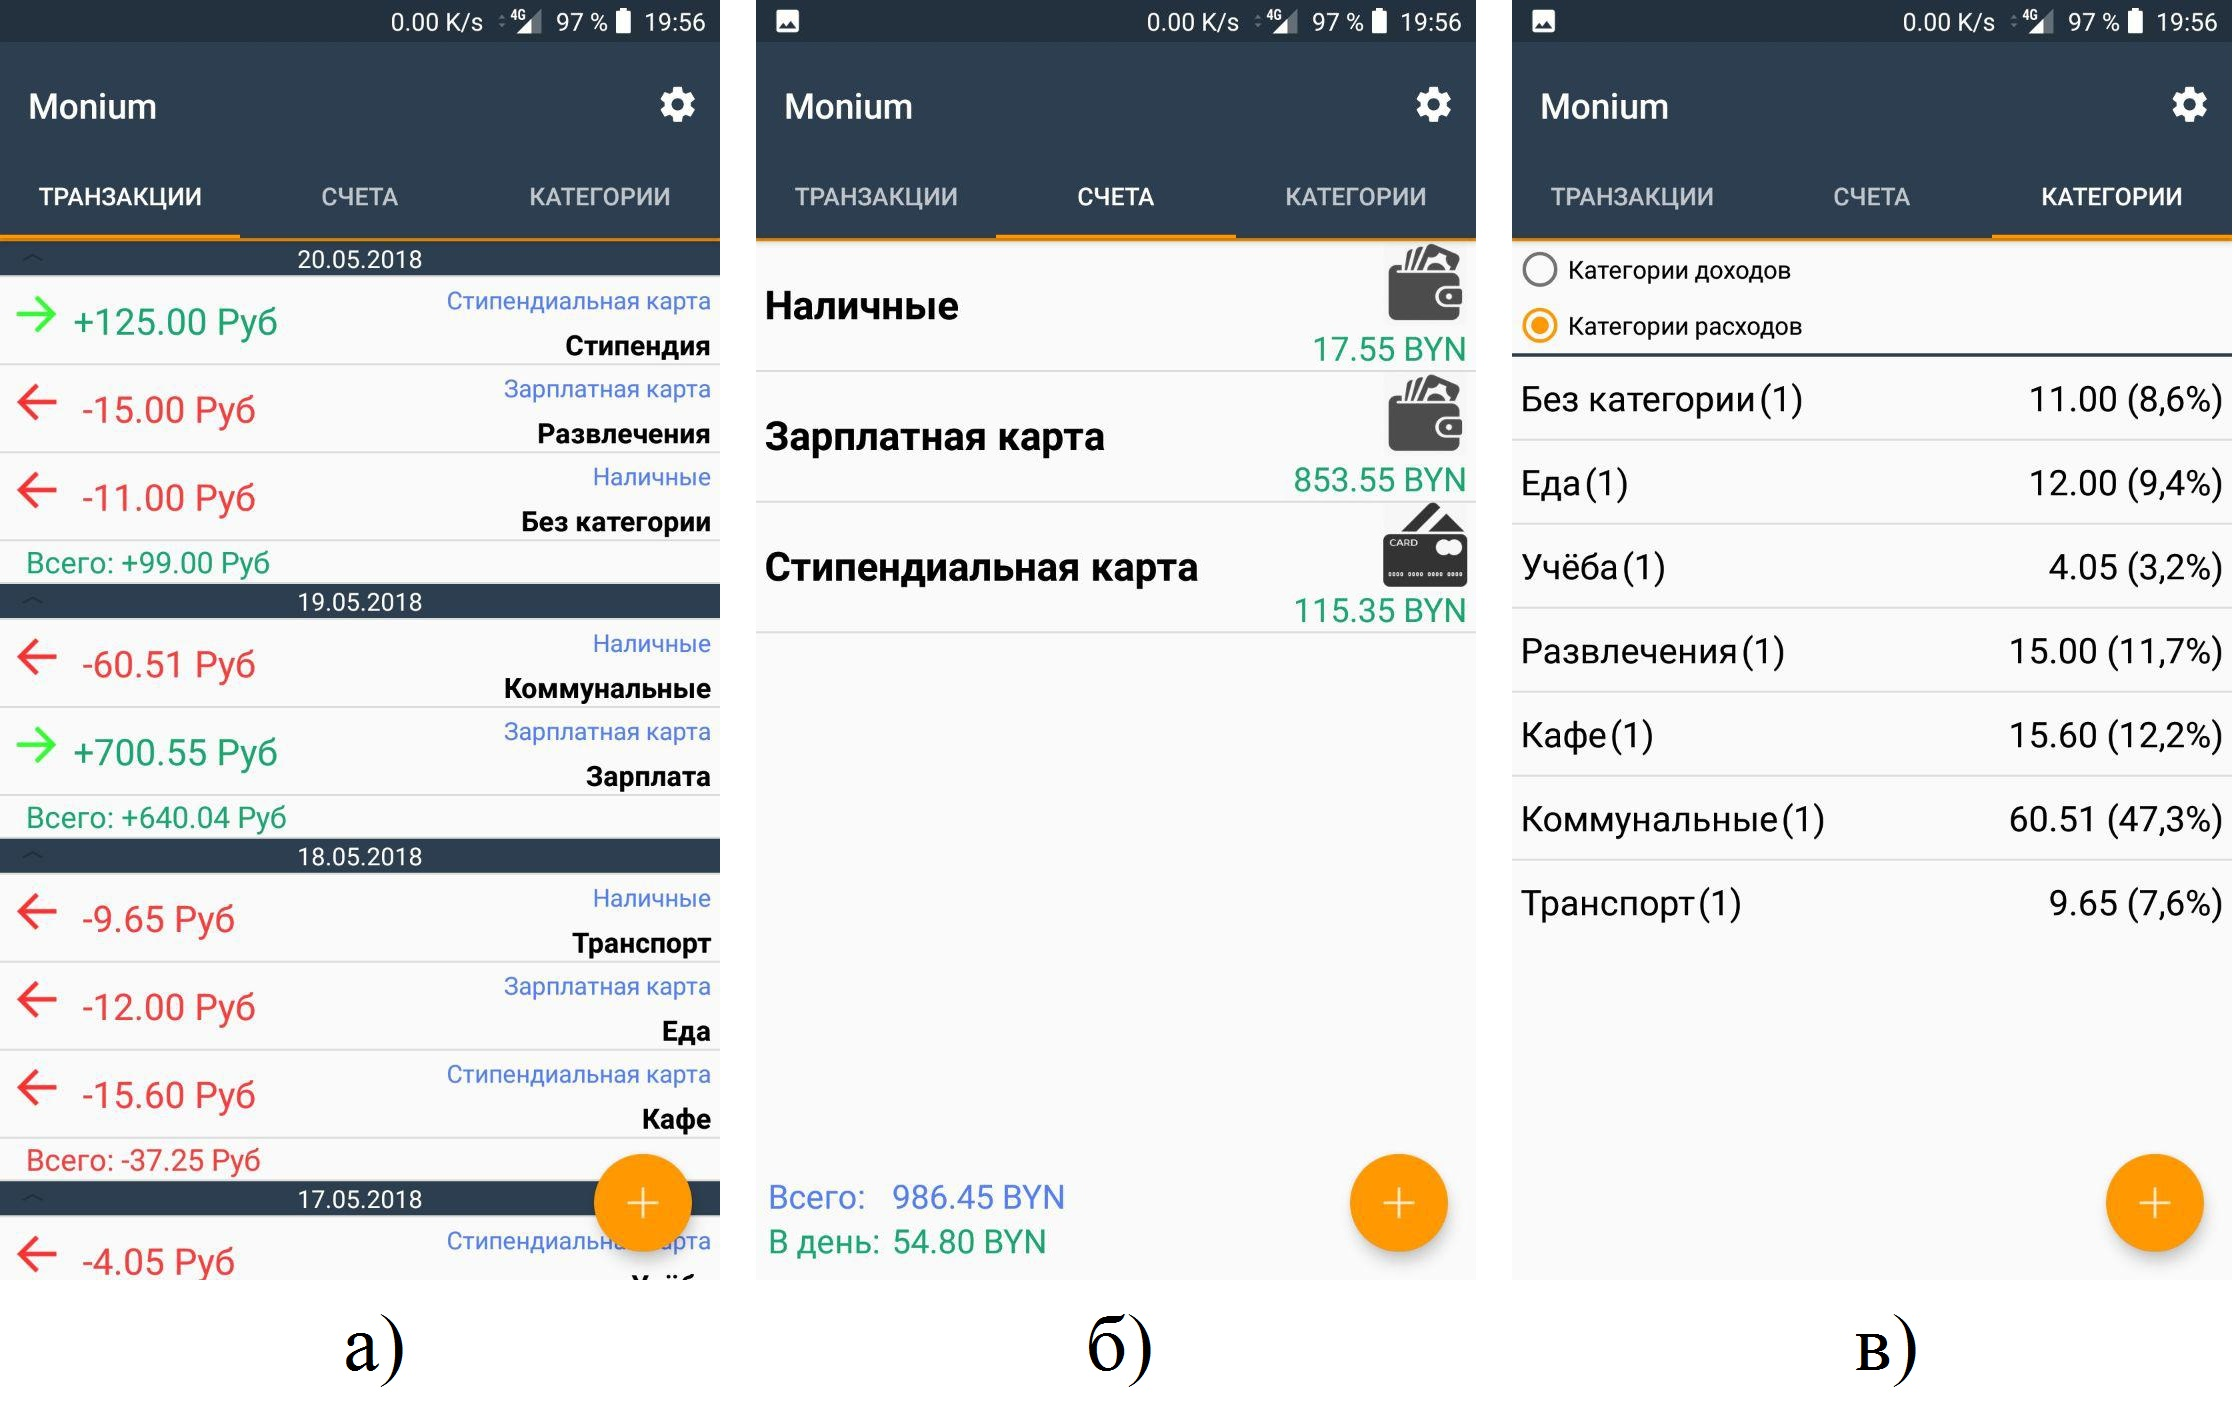
\includegraphics[scale=0.28]{5_1_lists.png}
    \caption{Экраны списков: а) -- список транзакций, б) -- список счетов, в) -- список категорий}
    \label{fig:manual:lists}
\end{figure}

При отсутствии каких-либо счетов, после нажатия на кнопку <<+>> появится сообщение <<Вы не добавили ни одного счёта>>.
Поэтому для начала требуется создать новый счёт: требуется переключиться на вкладку <<Счета>> и нажать на ту же оранжевую кнопку, однако откроется окно добавления счёта (см. рисунок~\ref{fig:manual:creates}б).
В данном окне следует ввести название счёта, остаток и выбрать валюту, также выбрать тип иконки счёта и нажать кнопку <<Добавить>>.
Процедура добавления транзакции отличается от процедуры добавления счёта только различиями в вводимых данных.
Из окна создания транзакции можно добавить счет или категорию через дополнительные кнопки <<+>> справа от каждого списка (см. рисунок~\ref{fig:manual:creates}а).

\begin{figure}[H]
    \centering
    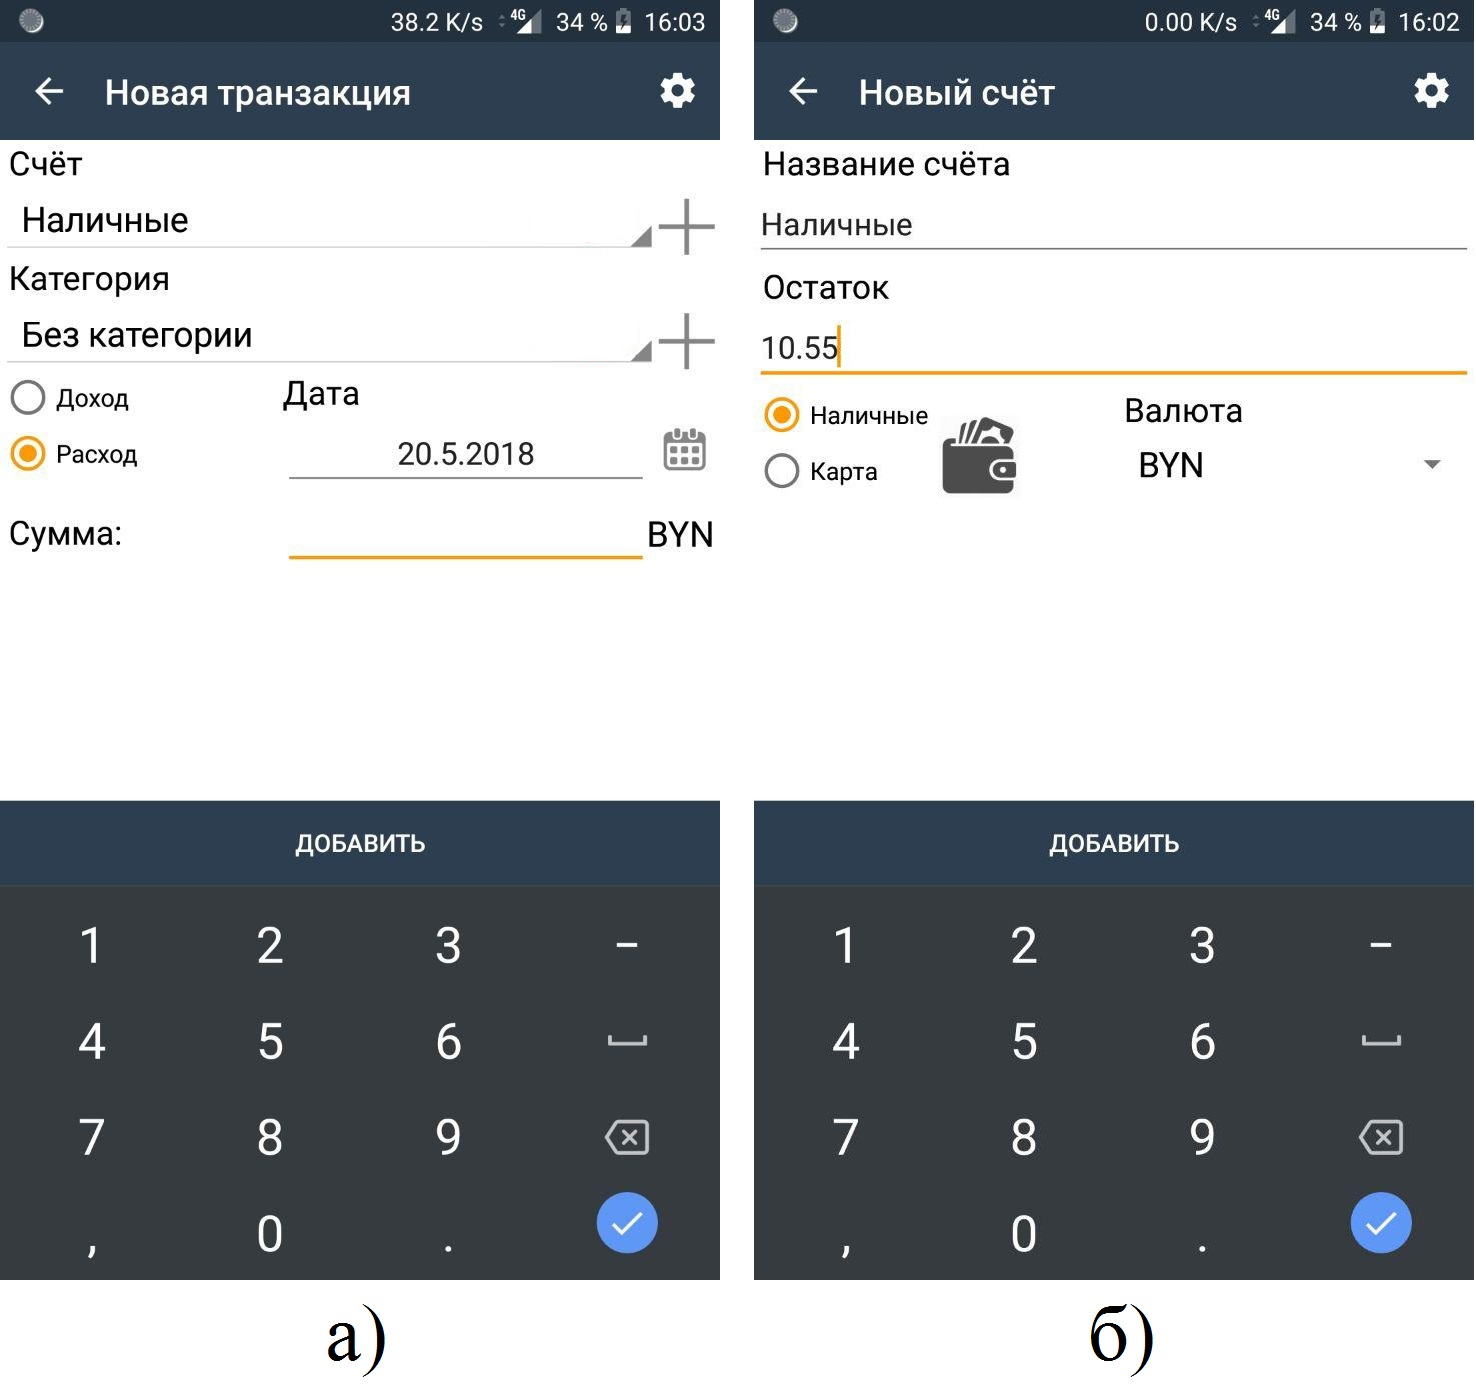
\includegraphics[scale=0.32]{5_2_creates.png}
    \caption{Формы создания сущностей: а) -- новая транзакция, б) -- новый счёт}
    \label{fig:manual:creates}
\end{figure}

В качестве даты по умолчанию устанавливается текущая системная дата, для смены даты требуется нажать на иконку календаря рядом с полем даты.

Для управления существующими транзакциями, счетами или категориями необходимо осуществить долгое нажатие на соответствующем элементе списка.
После нажатия отображается контекстное меню со списком доступных действий (см. рисунок~\ref{fig:manual:category_context}а).
При удалении категории присутствует выбор между удалением всех транзакций, связанных с этой категорией или смена этой категории во всех зависимых транзакциях на новую (см. рисунок~\ref{fig:manual:creates}б).
Пункт <<Отчистить статистику>> удаляет все транзакции, связанные с данной категории.

\begin{figure}[H]
    \centering
    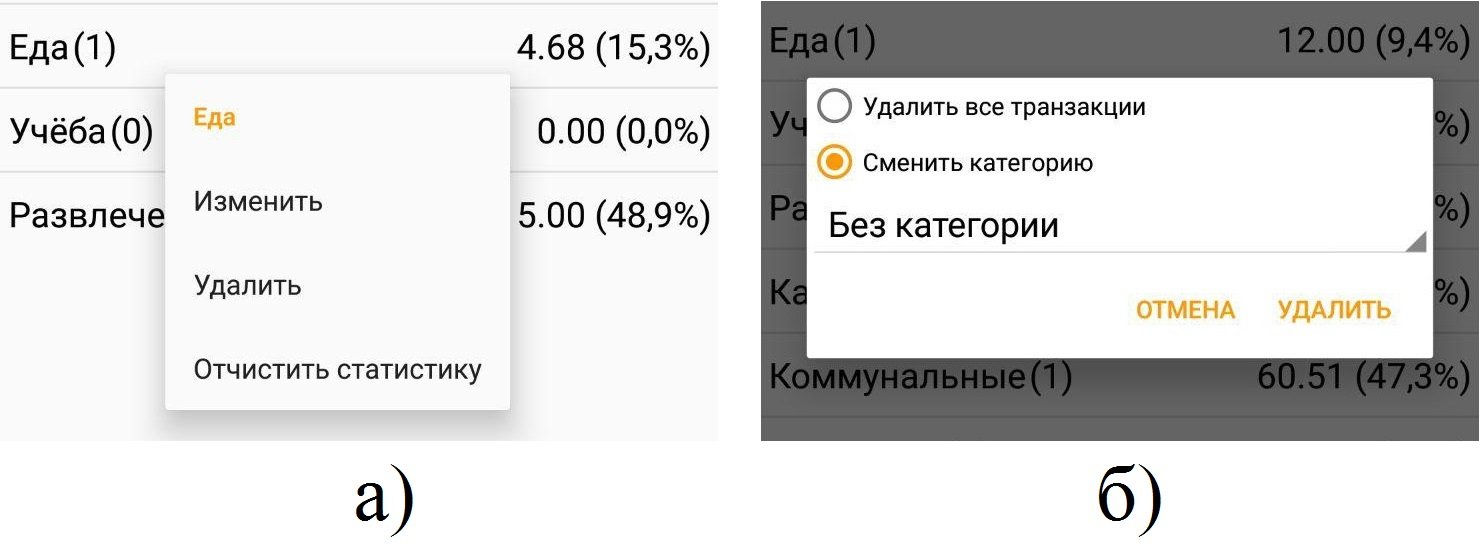
\includegraphics[scale=0.32]{5_3_category_context.png}
    \caption{Контекстные меню категории: а) -- список операций над категорией, б) -- меню удаления категории}
    \label{fig:manual:category_context}
\end{figure}

Таким образом, в данном разделе приведены примеры использования некоторых их основных возможностей разработанного программного средства.
Следование им должно значительно упростить выполнение некоторых рутинных задач учёта персонального бюджета.
